\documentclass{article}
\usepackage{graphicx} % Required for inserting images
\usepackage{float}
\usepackage{longtable}
\usepackage{caption}
\usepackage{setspace} 
\usepackage{lineno}
\usepackage{authblk}
\usepackage[margin=1in]{geometry}
\usepackage[
backend=biber,
style=apa,
sorting=nyt
]{biblatex}
\addbibresource{maintext.bib}

\title{An integrated integral projection model (IPM\textsuperscript{2}) to disentangle size-structured harvest and natural mortality}
\author[1,*]{Abigail G. Keller}
\author[2]{Benjamin R. Goldstein}
\author[3]{Leah Skare}
\author[1]{Perry de Valpine}
\affil[1]{\small Department of Environment Science, Policy, and Management, University of California, Berkeley, Berkeley, California, USA}
\affil[2]{\small Department of Forestry and Environmental Resources, North Carolina State University, Raleigh, NC, USA}
\affil[3]{\small Northwest Straits Commission (ADD MORE)}
\affil[*]{\small Corresponding author: Abigail G. Keller, agkeller@berkeley.edu}
\date{}

\begin{document}


\doublespacing

\linenumbers

\maketitle

\section{Abstract}

\textbf{Key words:} integrated population model, integral projection model, state-space framework, invasive species, European green crab, size structure

\newpage

\section{Introduction}

Assessing the efficacy of invasive species management interventions requires understanding if and how removal actions change population abundance and dynamics. However, population suppression can be challenging to differentiate from natural biological variation, reflecting the perennial challenge of distinguishing harvest and natural mortality in assessment of fishery stocks \parencite{aanes2007estimation}. Often variability in harvest mortality is confounded with variability in natural mortality \parencite{lewy2003modelling}, yet separating these fluctuations is crucial for obtaining reliable estimates of population abundance and demographic rates \parencite{walters2004fisheries}. Invasive species removal program success is highly variable \parencite{prior2018does}, so reliably quantifying harvest rates will be essential for defining intervention success and efficiently allocating limited management resources \parencite{green2021functional}.

This challenge of disentangling sources of mortality is amplified for species with complex, size-structured demography. Body size can be one of the most important traits of an individual organism, often determining the strength of ecological interactions and influencing key life-history processes like growth and mortality \parencite{de2003influence}. The ontogenetic scaling of ecological performance with body size has been used to explain patterns at the population level \parencite{werner1994ontogenetic}. Population dynamics can be shaped by competitive and predatory (cannibalistic) intra-specific interactions between different size cohorts \parencite{claessen2004population}, predator-prey size-dependent functional responses \parencite{aljetlawi2004prey}, variable reproductive capacity across size \parencite{hixon2014boffffs}, and size-selective rates of harvest \parencite{tu2018fishing}. Since these size-structured rates and interactions simultaneously modulate population dynamics, unraveling their individual contributions can be difficult. 

Removal sampling data are the primary source of monitoring information for many invasive populations \parencite{udell2022open}. Invasive species datasets are often collected opportunistically as part of removal programs, rather than experimentally designed, limiting inference about population demographic rates \parencite{tiberti2021alien, crall2010improving, rogosch2021comparing}. Multinomial N-mixture models can be used to estimate abundance with animals removed successively from multiple sites \parencite{dorazio2005improving}, yet these models make strict assumptions, like population closure and no other sources of mortality, that often opportunistic datasets do not meet. These removal observations are often not collected systematically across time and space and can be associated with large measurement error that can mask biological signals \parencite{auger2016state, sibert2003horizontal, katsanevakis2012monitoring}.

Despite the unique statistical inference challenges associated with invasive species removal data, the ecological, economic, and social costs of under- and over-estimating removal harvest rates can be high. Inefficient invasive population suppression plans can result in a waste of human and economic resources and can affect the confidence of people and stakeholders involved in removal \parencite{tiberti2021alien}. As invasive species management becomes more ambitious in scope and scale, population control can be controversial, stimulating conflicts among people and debates about achievability and efficiency \parencite{crowley2017conflict}. These undesirable social outcomes underscore the need for rigorous assessments of the effectiveness of control programs.

Combining existing classes of models can be useful for distinguishing process and observation dynamics, facilitating parameter identifiability, and enabling inference about complex, size-structured demographic rates from imperfect observations. First, an integral projection model can be used to make population projections based on individual-level, size-dependent vital rates \parencite{merow2014advancing, rees2014building}. In contrast to matrix population models with large data requirements, the integral projection model uses a kernel composed of continuous functions to describe the probability of transitioning between sizes \parencite{ellner2006integral}. The integral projection model can therefore substantially simplify inference by only requiring estimates of parameters in these continuous functions, rather than parameters to describe every possible size transition. 

The integral projection model can then be formulated in a state-space framework to estimate demographic rates with size-structured time series data \parencite{white2016fitting}. State-space approaches partition latent process model dynamics from both process and measurement error, providing a hierarchical structure that separately models 1) an unobserved, process time series that reflects the true, hidden population state and 2) an observation time series that contains imperfect measurements related to the process time series \parencite{auger2021guide}. By separating latent process model dynamics from both process and observation error, the state-space framework allows distinct estimation of harvest mortality — the observation process — from natural biological variation.

These state-space approaches, however, can suffer from challenges of parameter identifiability, especially in scenarios when information requirements of complex models exceed information available in a single dataset \parencite{auger2016state}. Integrated population models can resolve these identifiability issues by jointly analyzing multiple datasets in an integrated framework. By combining survey and demographic data, these models increase the precision of parameter estimates and facilitate estimation of “additional” parameters not identifiable with individual datasets \parencite{riecke2019integrated, abadi2010assessment}. By combining an integrated population model with an integral projection model – an integrated integral projection model (IPM\textsuperscript{2}) – the relationship between individual size and demographic performance can be used to forecast population-level processes \parencite{plard2019ipm}.

An integrated integral projection model (IPM\textsuperscript{2}) will be useful for understanding size-structured population dynamics and removal effectiveness of invasive European green crab (\textit{Carcinus maenas}). Listed as one of the world’s 100 worst invaders \parencite{lowe2000100}, the European green crab has successfully colonized all continents except Antarctica \parencite{yamada2001global}, negatively impacting benthic communities \parencite{grosholz2005recent}, eelgrass habitat \parencite{garbary2014drastic, howard2019habitat}, and commercial shellfish industries \parencite{grosholz2011modeling}. The European green crab is a resilient marine invader, largely because of a mismatch in spatial scale between local removal programs and the crab’s wide-ranging dispersal and population processes \parencite{keller2025transition}. While adult crabs occupy sheltered bays and estuaries, the crab’s dispersal larval phase in open marine waters often facilitates recolonization of suppressed populations from neighboring habitats \parencite{yamada2021ocean}. Understanding the relationship between removal effort and population suppression will therefore be critical for identifying the feasibility of suppression and for efficiently allocating conservation resources. 

The green crab’s local dynamics are regulated by complex, size-structured demography. Adult crabs exert direct control of recruitment, largely through strong negative adult-juvenile interactions (i.e., cannibalism) \parencite{grosholz2021stage, romano2017cannibalism}. Competition with native crabs is also size-structured, with larger crabs maintaining a competitive advantage for space and resources \parencite{mcdonald2001competitive, jensen2007biotic}. Importantly, these individual, size-structured interactions modulate population-level processes; a field experiment in California, USA found a 30-fold, single-year increase in total green crab abundance in response to removal \parencite{grosholz2021stage}. This high level of juvenile survival associated with low adult abundance, often referred to as overcompensation or the "hydra effect", underscores the importance of quantifying size-structured population response to removal (Abrams 2009). 

The green crab observation process is also size-selective, further complicating distinction between simultaneous size-structured processes. Common in marine systems, many green crab size classes are completely unobserved, as baited traps used for removal do not catch all individuals with equal probability across size classes \parencite{jorgensen2009size}. Additionally, the observability of the population changes within a trapping season as individuals grow into size classes capable of being caught in traps. Quantifying the relationship between removal effort and size-structured removal rates will be necessary for assessing the feasibility and impact of removal, understanding long-term dynamics, and optimizing management actions and decisions for this high priority species. 

Here we develop an integrated integral projection model (IPM\textsuperscript{2}) to quantify size-structured harvest rates of invasive European green crab. As part of a state-space framework, process dynamics are described using an integral projection model, where the population structure changes over time through seasonal growth, natural mortality, and removal, and observations are generated through the use of multiple size-selective removal methods (Figure 1). Combining multiple datasets in an integrated framework allows for distinct inference about size-structured harvest and natural mortality rates, “additional parameters” for which no explicit data is collected (Figure 2). The IPM\textsuperscript{2} facilitates prediction of the stable size distribution and equilibrium abundance under different removal strategies, providing a framework for accurate assessment of the effectiveness of invasive species control programs.

\section{Methods and materials}

\subsection{Demographic data}

Population-level inference is focused on size-structured green crab abundance at Drayton Harbor in Washington, USA (Appendix 1.1, Figure A1.1). Data were collected from 2020-2023, with an intra-annual time series of size-structured removal count observations (D1, Figure 1B). Multiple trap types (Fukui, Minnow, and Shrimp) with different size-selective removal rates were used (Figure 1B), and traps were baited and left to "soak" in intertidal and subtidal habitat for 24-48 hours. Drayton Harbor is an enclosed bay, and we assume no movement in and out of the study site within each year. 

Inference was supplemented by two additional datasets, size-at-age data (D2) and batch mark-recapture data (D3). Size-at-age data (D2) were collected from two sources: 1) records from crab removal observations in northeastern Pacific estuaries from Yamada et al. 2005, when the somatic growth of a strong recruitment class was tracked over time, and 2) crabs with an assigned age from Drayton Harbor that were easily identifiable based on size and carapace color \parencite{yamada2005growth}. While data from these Drayton Harbor recruits entered the integrated population model likelihood twice (D1 and D2), extensive simulation-based research has revealed that IPMs are robust to dependent data \parencite{abadi2010assessment}. Size-structured batch mark-recapture data (D3) was collected by Grosholz et al. 2021 in a mark-recapture experiment in Seadrift lagoon, California, USA \parencite{grosholz2021stage}. Here, green crabs were captured, marked, and released with Fukui traps and then recaptured within a few weeks, and batch markings do not allow individual identification. 

More information on all three datasets can be found in Appendix 1. 

\subsection{Model description}

We start by detailing the overall state-space population model, including the process and observation sub-models (Figure 1). We then describe how the parameters of the model are informed by the different datasets. Description of all model parameters can be found in Table 1.

\subsubsection{Process model}

The process model describes how unobserved, latent states depend on past states \parencite{auger2021guide}. The following process equations describe the initial adult population size and annual recruitment, as well as the growth and survival kernel that projects the population forward in time based on seasonal size-dependent growth and size-dependent natural survival \parencite{rees2014building}. These equations describe how the population changes within a year (intra-annual change) and between years (inter-annual change) (Figure 1). The model tracks the state of the population in terms of its distribution of carapace sizes, $N_{t, i, y}$, which is the density function of individuals of size $y$ during year $i$ at time $t$. 

\subsubsection*{Initial population density and annual recruitment}

The initial size distribution, $N_{t=1, i=1, y}$, is a function of the abundance of adults at the first time period during the first year, $\lambda^{A}$, the mean initial adult size in millimeters, $\mu^A_{y}$, and the standard deviation of initial adult size in millimeters, $\sigma^A_{y}$. $f_L$ represents the log-normal probability density function.

\begin{equation}
N_{t=1, i=1, y} = f_L(y; \mu^A_{y}, \sigma^A_{y}) \times \lambda^A
\end{equation}

Ovigerous females spawn in August-December \parencite{klassen2007biological}, and these planktonic larvae exit estuarine habitat to develop in high salinity coastal waters alongside larvae produced by neighboring habitats. Advection then brings larvae back into the estuary during recruitment \parencite{young2019life}. Reproduction is therefore modeled as an annual event with open demography, where the annual abundance of recruits, $\lambda^R_i$, is independent of adult abundance and follows a normal distribution, truncated such that $\lambda^R_i > 0$  

\begin{equation}
\lambda^R_i \sim Normal(\mu^R_{\lambda}, \sigma^R_{\lambda})
\end{equation}

The annual size distribution of recruits, $R_{i, y}$, is a function of the annual abundance of recruits, $\lambda^R_i$, the mean initial recruit size in millimeters, $\mu^R_y$, and the standard deviation of initial recruit size in millimeters, $\sigma^R_y$. $f$ represents the normal probability density function.

\begin{equation}
R_{i, y} = f(y; \mu^R_{y}, \sigma^R_{y}) \times \lambda^R
\end{equation}

Most crabs will settle from their planktonic larval stage in January to April \parencite{yamada2005growth}. The recruits therefore enter the process model in mid-May, corresponding to $t=6$, when it can be assumed $\mu^R_y > 0$, yet before they grow into an observable size (Figure 1B).

\begin{equation}
N_{t=6, i, y} =  N_{t=6, i, y} + R_{i, y}
\end{equation}

\subsubsection*{Integral projection model}

The population density is then projected forward in time using an integral projection model (IPM). The IPM uses a continuous distribution over $y$, and the abundance of individuals is discretized using a small size interval $\Delta y$ centered on size $y$. The total population size, $N_{i,t}$ is $\int_{\Omega} N_{i,t,y} dy$, where $\Omega$ represents all biologically feasible sizes.

A kernel, $K(y', y, T)$, describes the probability density of moving from size $y$ to size $y'$. This kernel is time-dependent, where $T = [D(t), D(t+1)]$, a vector of calendar dates associated with $t$ and $t+1$. $N_{t+1,i,y}$ is therefore a function of $N_{t,i,y}$, $K(y', y, T)$, and the removed crabs, $n^R_{t,i,y}$

\begin{equation}
N_{t+1,i,y} = \int_{\Omega} K(y',y, T) (N_{t,i,y} - n^R_{t,i,y}) dy 
\end{equation}

In contrast to matrix population models with discrete size bins and transition probabilities between each size pair \parencite{caswell2001matrix}, the kernel is defined as a combination of functions that are continuous over size $y$. The kernel is the product of a growth kernel, $G(y',y, T)$, and size-dependent natural survival, $S(y)$:

\begin{equation}
K(y',y, T) = G(y',y, T) \times S(y)
\end{equation}

\subsubsection*{Seasonal growth}

Like many ectotherms, green crab growth is strongly seasonal, with the growth rate peaking in the summer due to seasonal variation in temperature, light, and food availability \parencite{contreras2003population, garcia2012technical}. We therefore use a seasonal growth model that modifies the traditional von Bertalanffy growth model proposed by Beverton and Holt \parencite{beverton2012dynamics, somers1988seasonally}.

\begin{equation}
\mu^G_{y,T} = y + (y_{\infty}-y)(1-exp(-k\Delta t-S_t+S_{t0}))
\end{equation}
\begin{equation}
S_t = \frac{Ck}{2\pi} sin(2\pi(D(t+1)-t_s)
\end{equation}
\begin{equation}
S_{t0} = \frac{Ck}{2\pi} sin(2\pi(D(t)-t_s)
\end{equation}

where $\mu^G_{y,T}$ is the mean size at $t+1$, $y_{\infty}$ is the asymptotic average size, $k$ is a measure of the exponential rate of approach to the asymptotic size, $C$ modulates the amplitude of the growth oscillations, and $t_s$ is the time between the start of the calendar year and the start of the convex portion of the first sinusoidal growth oscillation \parencite{garcia2012technical}.

To account for variation in growth rate among individuals, $G(y',y, T)$ is described as:

\begin{equation}
G(y',y=x, T) = f(y'; \mu^G_{y=x, T}, \sigma^G)
\end{equation}

\subsubsection*{Natural mortality}

The rate of natural mortality decreases with size, as smaller crabs have lower intra- and inter-specific competitive abilities and are more susceptible to predation and cannibalism \parencite{maszczyk2018body, grosholz2021stage}. Natural survival, $S$, is described as: 

\begin{equation}
S(y)_i = exp(-\Delta t(\beta_i+\frac{\alpha}{y^2}))
\end{equation}

where $\beta$ is the intensity of size-independent natural mortality and $\alpha$ is the intensity of size-dependent natural mortality \parencite{carlson2010bayesian}. Here, process error enters the model as year-specific, size-independent natural mortality:

\begin{equation}
\beta_i \sim Gamma(\beta_{\alpha}, \beta_{\theta})
\end{equation}

\subsubsection*{Density-dependent overwinter mortality}

To transition from year $i$ to year $i+1$, the population density experiences seasonal growth and density- and size-dependent overwinter survival. The abundance of crabs surviving the winter, $N_{t=1,i+1,y}$, is drawn from a binomial distribution, where $size$ is the abundance of crabs after seasonal growth and removal in the last time period, $t_{max}$, and $p$ is the probability of overwinter survival, $S^o_{y,i}$. Here $T=[D(t=t_{max}), D(t=1)]$. 

\begin{equation}
N_{t=1,i+1,y} \sim Binomial( \int_{\Omega} G(y',y, T) (N_{t_{max},i,y} - n^R_{t_{max},i,y}) dy,  S^o_{y,i})
\end{equation}

Due to thermal stress and starvation, the intensity of overwinter mortality is likely stronger than other times of the year and plays an important role in population regulation through density-dependent control on population size \parencite{henderson1988size}. Overwinter mortality is also size-selective; smaller animals tend to have lower energy reserves than larger animals and use reserves more rapidly due to the allometry of metabolic rate \parencite{hurst2007causes}. Probability of overwinter survival, $S^o$, is therefore modeled as a density-size interaction, such that the intensity of size-dependent overwinter mortality increases at higher population densities. $N^T_{t_{max},i}$ is the total abundance at site $i$ at the onset of winter.

\begin{equation}
S^o(y,N^T_{t_{max},i}) = exp(-\frac{\alpha_i^o \times N^T_{t_{max},i}}{y^2})
\end{equation}

Process error enters as a year-specific strength of density- and size-dependent overwinter mortality.

\begin{equation}
\alpha^o_i \sim Gamma(\alpha^o_{\alpha}, \alpha^o_{\theta})
\end{equation}

\subsubsection{Observation model}

\subsubsection*{Conditional multinomial observation model}

A conditional multinomial observation model is used to describe the data-generating process for the removal count data $n^C_{t,i,y,j}$, representing the number of crabs of size $y$, caught at time $t$, during year $i$, in trap $j$ (Figure 1) \parencite{kery2015modeling}. Multiple traps are placed simultaneously at each time period, so this method breaks the observation model into two pieces: 1) a binomial with an unknown sample size, the total abundance of crabs, $N_{t,i,y}$, and 2) a multinomial conditioned on a known sample size, the total number of removed crabs across all traps in each time period, $n^R_{t,i,y}$.

The total number of removed crabs, $n^R_{t,i,y}$, follows a binomial distribution with the total abundance of crabs, $N_{t,i,y}$, and total capture probability, $p_{t,i,y}$.

\begin{equation}
n^R_{t,i,y} \sim Binomial(N_{t,i,y}, p_{t,i,y})
\end{equation}

The size-structured count of crabs in each trap, $n^C_{t,i,y,j}$, follows a multinomial-dirichlet mixture distribution where the probability of capture in trap $j$, $p^C_{t,j,i,y}$, is conditioned on being captured at all, $p_{t,i,y}$. Since the trap compositional data are overdispersed due to green crab aggregation and spatial behaviors, the dirichlet allows for greater variance in the count data than predicted by a multinomial distribution \parencite{thorson2017model}. The observed conditional probability of capture, $p^C_{t,j,i,y}$, therefore varies from the mean conditional probability of capture, $\tilde{p}^C_{t,j,i,y}$. More information on the multinomial-dirichlet mixture can be found in Appendix 2.2.

\begin{equation}
n^C_{t,j,i,y} | n^R_{t,i,y} \sim Multinomial(n^R_{t,i,y}, p^C_{t,j,i,y}|\tilde{p}^C_{t,j,i,y})Dirichlet(\tilde{p}^C_{t,j,i,y}| \alpha^D_{t,j,i,y})
\end{equation}

\subsubsection*{Size-selective hazard rates}

Harvest mortality through trapping occurs in continuous time, described as a size-selective hazard rate, $H(y)$, representing the instantaneous intensity of capture (Ergon 2018). The shape and magnitude of this size-selective hazard rate varies among the three trap types used for removal: Fukui, Minnow, and Shrimp traps.

Both Fukui and Shrimp traps capture larger crabs at higher rates than smaller crabs. The hazard rates, $H_F(y)$ and $H_S(y)$, of these trap types are a logistic function of crab size:

\begin{equation}
H_F(y) = \frac{h^{max}_F}{1+e^{-h^k_F(y-h^0_F)}}
\end{equation}
\begin{equation}
H_S(y) = \frac{h^{max}_S}{1+e^{-h^k_S(y-h^0_S)}}
\end{equation}

The Minnow trap mesh size is smaller than the maximum crab size, so the size-selective hazard rate follows a bell-shaped curve \parencite{jorgensen2009size}.

\begin{equation}
H_M(y) = h^{max}_M \times exp(\frac{y-h^{A}_M}{2 h^{\sigma}_M})
\end{equation}

Each baited trap, $j$, is placed in the habitat for a short ($\sim$24-48 hrs) time interval, $\Delta b_{t,i,j}$. The probability of surviving trap mortality, $S_{t,i,y}$, is the integrated hazard rate, summed across all traps set during the same time period, $O_{t,i}$.

\begin{equation}
S_{t,i,y} = exp(-\sum_{j=1}^{O_{t,i}} H_{t,j,i,y}\Delta b_{t,i,j})
\end{equation}

The total capture probability, $p_{t,i,y}$, is described as the probability of not surviving the trapping time interval, $p_{t,i,y} = 1-S_{t,i,y}$. The mean conditional probability of capture, $\tilde{p}^C_{t,j,i,y}$, is then $H_{t,j,i,y}/\sum_{j=1}^{O_{t,i}}H_{t,j,i,y}$.

\subsubsection*{Integrated population model}

We combined the population data from three data sources to jointly estimate demographic parameters, observation parameters, and latent states (Figure 2; Table 1). The size-at-age data (D2) directly informed the seasonal growth parameters. Inference was conducted sequentially, such that the seasonal growth parameters were fit with the size-at-age records, and the summarized posteriors were used to develop prior distributions in the overall IPM. More information on model fitting with D2 can be found in Appendix 1.2. 

The mark-recapture data (D3) primarily informed the observation parameters that describe the size-selective hazard rates of the Fukui trap type, although these data also informed components of the growth and natural mortality kernel (Table 1; Figure 2). Inference using the time series data (D1, Figure 1B) and mark-recapture data (D3) was performed simultaneously, with both datasets entering the likelihood as data, rather than priors. The state-space model was therefore augmented with the following equations to integrate the mark-recapture data (D3).

The number of marked and released crabs of size $y$, $n_y^{mc}$, at $t_1^{mc}$ underwent seasonal growth and natural mortality to the next time period, $t_2^{mc}$.

\begin{equation}
n_{y,t_2}^{mc} = \int_{\Omega} K(y',y, T^{mc}) n_{y,t_1}^{mc} dy 
\end{equation}

The number of recaptured and marked crabs of size $y$ at $t_2^{mc}$, $m_{y}^{mc}$, follows a binomial distribution:

\begin{equation}
m_{y}^{mc} \sim Binomial(n_{y,t_2}^{mc}, p_y^{mc}) 
\end{equation}

where $p_y^{mc}$ is the total probability of capture based on the total number of Fukui traps set, $O^{mc}$, over the time period $\Delta b^{mc}$:

\begin{equation}
p_y^{mc} = 1-exp(-\sum_{j=1}^{O^{mc}}\int H_F(y)\Delta b^{mc})
\end{equation}


\subsection{Model fitting}
We fitted the integrated integral projection model in a Bayesian framework using NIMBLE v.1.2.1 \parencite{de2017programming}. We used vague priors for all parameters, which are provided in Appendix 2.1. Parameters were estimated by running four Markov chain Monte Carlo (MCMC) chains of 100 000 iterations, thinned by a factor of 10. Of the remaining 10 000 samples, 2 000 were discarded as burn-in. We used visual inspection of the MCMC chains and the Brooks and Gelman diagnostic $\hat{R}$ to assess model convergence, and we found that all parameters had an $\hat{R} \leq 1.05$ \parencite{brooks1998general}. All analyses were conducted in R v.4.41 \parencite{Rcore}. Code for the entire model is provided in Appendix 3, and generic, modular code that closely follows the model description is provided in Appendix 4. Posterior summaries, as well as convergence diagnostics and trace plots of model parameters can be found in Appendix 5.

To assess model performance and robustness, we conducted both a model selection and a model checking procedure \parencite{conn2018guide}. For model selection, we evaluated multiple functional forms of overwinter mortality using Watanabe–Akaike information criterion (WAIC). The inter-annual population transitions (i.e., transition from year $i$ to year $i + 1$) are largely described by density-dependent overwinter mortality. Since density dependence only enters the model during this process and is therefore likely influential for forecasting the stable size distribution, we compared multiple functional forms for size- and density-dependent overwinter mortality and used the formulation with the lowest WAIC in the final analysis (Eq. 15-16, Appendix 6.1).

To check the model, we calculated posterior predictive p-values using the deviance as an omnibus discrepancy function and proportion of zeros as a targeted discrepancy function to check for zero inflation of the count data (Appendix 6.2). We found that the model was an adequate representation of the data-generating process, with p-values of 0.92 for both the deviance and proportion of zeros discrepancy functions (Appendix 6.2; Figures A.6.1 and A6.2).


\subsection{Population forecasts}

To evaluate how a green crab population responds to varying removal efforts, we calculated the stable size distribution and equilibrium abundance through stochastic forward simulations with posterior samples. We randomly selected 1000  samples from the full posterior, and for each posterior sample, we generated an initial adult population size and projected the population forward 25 years, applying varying removal efforts for each set of 1000 simulations. These varying removal efforts included a total of 0, 28, 112, 560, 840, 1400, and 2800 annual Shrimp, Fukui, or Minnow traps, applied evenly over the trapping season of 14 biweeks (21 total sets of 1000 simulations; seven removal efforts x three trap types). Year-varying quantities, like recruit abundance, size-independent natural mortality, and size- and density-dependent overwinter mortality were drawn stochastically each year in the forward simulations (Table 1). To ensure proper comparisons between removal effort and trap type combinations, the same set of year-varying stochastic draws for each posterior sample was consistent across the 21 simulation sets. 

For each simulation, $S$, the size-structured abundance at the end each of year after overwinter mortality, $N_{t=1,i+1,y}$, was recorded (Figure 1A). Simulation outputs were summarized as the mean size-structured abundance at the end of years 6-25, as the first five years were discarded as burn-in to ensure the population reached an equilibrium.

\section{Results}

\subsection{Estimating population-level quantities}

The integrated population model tracked the size-structured European green crab abundance at Drayton Harbor (D1) throughout 2020-2023. Figure 3 shows the population density of adults and recruits at the beginning of each year (Figure 3). As the invasion progressed from 2020 to later years in 2021-2023, the size structure of adults shifted toward larger crab sizes (Figure 3A). This increase in median adult crab size coincided with a decrease in overall adult crab abundance. Total adult crab abundance decreased from 335 (274-430 95\% CrI) individuals in 2020 to 250 (238-266 95\% CrI), 154 (146-164 95\% CrI), and 165 (154-183 95\% CrI) in 2021-2023. The size distribution of adults in 2021-2023 is also bimodal, as the recruit age class that survived the winter (year one class) had not yet grown in size to match the sizes of crabs older than one year.

The abundance of recruits varied by multiple orders of magnitude across years, ranging from 528 (253-969 95\% CrI) and 1105 (668-1669 95\% CrI) in the strong recruitment years of 2020 and 2022, to 42 (29-58 95\% CrI) and 54 (20-102 95\% CrI) in the weak recruitment years of 2021 and 2023 (Figure 3B). 

\subsection{Distinguishing size-structured natural and harvest mortality}

By combining information in multiple datasets, the integrated population model allowed for estimation of "additional" parameters -- size-structured natural and harvest mortality -- that were not identifiable with the component datasets \parencite{riecke2019integrated}.

Removal rates were estimated for three trap types -- Fukui, Shrimp, and Minnow -- with different rates of removal and size-selectivities (Figure 4). Overall, Shrimp traps removed crabs at the highest rate, and Minnow traps were only effective at removing crabs in the 30-60 mm size range. All traps do not effectively remove crabs smaller than 30 mm, consistent with the completely unobserved small crab portion of the population (Figure 1B).

Overwinter natural survival rates were lower than natural survival rates at other periods of the year (Figure 5), consistent with the expectation that overwinter mortality plays an important role in population regulation. Overwinter survival rates were also density-dependent and corresponded to the recruitment strength: in the winters between 2020 and 2021 and between 2022 and 2023 -- two years with the highest recruitment rates -- the overwinter survival rates were lower.

Overwinter mortality varied significantly from year to year, and years with higher overall population density coincided with particularly low overwinter survival of small crabs (Figure 5B). In response to a large recruitment event in 2022 (Figure 3), between 2022 and 2023, overwinter survival rates dropped to 0.6 for crabs of the largest size and less than 0.2 for crabs of smaller size (Figure 5B). Conversely, survival rates were high over the winter between 2021 and 2022 in response to a small recruitment event in 2021 (Figure 3B) and an adult size structure biased toward larger crabs (Figure 3A). 

\subsection{Population forecasts}

Forward simulations with posterior samples were used to forecast the stable size distribution and equilibrium abundance under different levels of removal effort, and subsequently different levels of removal mortality (Figure 6; Figure S1). These simulations indicated that a low removal effort with Fukui and Minnow traps (Figure 6B-C) resulted in only marginal changes in the stable size distribution and equilibrium abundance relative to no removal effort (Figure 6A). Large adult crabs can be completely removed from the population with a high removal effort of Shrimp traps (Figure 6D), but this large crab removal shifts the stable size distribution toward smaller crabs, as the equilibrium abundance of smaller crabs increases relative to no removal effort (Figure 6; Figure S2).

\section{Discussion}

Our integrated integral projection model (IPM\textsuperscript{2}) – a framework first described by Plard et al. 2019 – provides important insight for how body size can modulate many individual-level demographic rates that interact to describe population-level dynamics \parencite{plard2019ipm}. The IPM\textsuperscript{2} produces an outcome greater than the sum of its parts: combining information in multiple datasets facilitates population inference for a species with complex demography with imperfect measurements. We are able to disentangle multiple size-structured demographic rates that simultaneously change the size distribution over time \parencite{sogard1997size, carlson2010bayesian}, allowing detailed understanding of the individual contributions of each size-structured demographic rate to overall population dynamics. These results also fill a significant knowledge gap for invasive European green crab (\textit{Carcinus maenas}). While the species is highly studied due to its geographic ubiquity and management concern, this study is the first to quantify removal rates and size-structured population abundance \parencite{young2019life}, providing a path forward for assessing feasibility of control and optimizing management actions.

\subsection{Disentangling size-structured demographic rates}

The IPM\textsuperscript{2} provides novel insights into previously uncharacterized size-structured European green crab demographic rates, including size-structured natural mortality, size- and density-dependent overwinter mortality, recruitment processes, size-structured growth rate, and size-selective harvest rates. 

The model estimates unobserved quantities, most notably the abundance and size (carapace width) of recruits before they grow into observable size classes (Figure 1B, Figure 3). Due to the size-selectivity of most observation and removal methods, very little is known about early stages of the green crab life cycle \parencite{yamada2005growth}, yet here, we used growth rates estimated by larger sizes to back-calculate size and abundance of recruits before they are observed. However, the model may underestimate non-overwinter natural mortality at smaller sizes, and therefore recruit abundance, because after settlement from the planktonic phase, recruits are unobserved for months and are likely dying naturally at very high rates (Figure 5A). Previous studies have reported extremely high densities of small juveniles (200-2000/m\textsuperscript{2}) when counting individuals within quadrats in the intertidal zone at low tide where most juveniles are found \parencite{breteler1976settlement, thiel1994recruitment}. Future work should integrate trap data with measurements of small crabs made by other means to improve estimates of size-dependent, non-overwinter natural mortality.

Overwinter mortality is a major size-selective process for green crab, as both energy reserves and metabolic rate scale with body size, such that larger individuals have higher energy reserves but lower metabolism and are therefore more resilient to starvation and physical extremes \parencite{carlson2008seasonal, sogard1997size}. Our results provide support for the hypothesis that crab size and overall population density interact to modulate overwinter mortality (Appendix 6.1). Overwinter mortality varied significantly from year to year, and years with higher overall population density coincided with particularly low overwinter survival of small crabs (Figure 5B). Overwinter mortality therefore plays an important role in regulating size-structured green crab population dynamics \parencite{henderson1988size}. 

Recruitment varies by orders of magnitude from year to year, ranging from about 50 recruits in weak years to 500-1000 in strong years (Figure 3B). The green crab has a long planktonic larval stage, living in open marine waters for months before advection back into the estuarine environment where they settle in the sub- and inter-tidal zone \parencite{yamada2001global}. This inter-annual variability in recruitment is consistent with varying oceanographic conditions; the survival and successful transport of larvae often coincide with oceanographic conditions like El Niño/Southern Oscillation (ENSO) and Pacific Decadal Oscillation (PDO) events \parencite{yamada2021ocean}. Though drawing from a small sample size of only four years, recruit abundance appears to be decoupled from adult abundance; for example, adult abundance was highest in 2020, yet recruit abundance was lowest in 2021 (Figure 3). These results suggest that recruitment is likely driven by oceanographic conditions and regional population dynamics, rather than local adult abundance. 

The model also estimates demographic rates that vary across time and size. Marine invertebrates are often subject to seasonal variation in environmental factors like photoperiod, food availability, and temperature, resulting in elevated rates of growth, feeding, and oxygen consumption in the summer season \parencite{brockington2001relative}. Consistent with this expectation, we find that green crab growth is strongly seasonal, with growth rate peaking in summer months and approaching zero in the winter (Appendix 1, Figure A1.2). Green crab growth rate is also size-dependent, as the molting rate is much higher at smaller crab sizes, and slows down as crabs approach the mean asymptotic crab size \parencite{yamada2005growth}.

The IPM\textsuperscript{2} estimates absolute size-selective capture rates for different trap types, allowing for the first estimates of size-structured abundance of European green crab (Young 2020). These capture rate and abundance estimates mark an important advance for moving beyond catch per unit effort (CPUE) as the primary, yet imperfect, method for measuring population trends \parencite{harley2001catch}. These results also highlight the strong size-selectivity of removal methods, since capture rates approaching zero for crabs smaller than 30 millimeters (Figure 4). This size selectivity will have uncertain evolutionary consequences, yet resolving this uncertainty will be important for projecting long-term population dynamics. Fishing-induced life-history evolution is frequently observed in harvested species \parencite{enberg2012fishing}, and previous invasive species management programs have demonstrated rapid ecological and evolutionary changes in response to selective harvesting, including a shift toward earlier size at maturity and an overall slower growing phenotype \parencite{evangelista2015impacts}. These phenotypic responses to removal programs can have strong effects on ecosystem recovery and therefore should be considered invasive species management \parencite{zavorka2020phenotypic}.

While the IPM\textsuperscript{2} is able to represent many simultaneous size-structured demographic rates, the model specification may contain un-modeled heterogeneity in capture probability. To account for the spatial aggregative behavior of green crab, we used a Dirichlet-multinomial mixture to account for overdispersion (i.e., inflation of zeros in count data) across traps set simultaneously \parencite{thorson2017model, young2019life}. However, the presence of large crabs or large numbers of crabs can also dissuade additional crabs from entering a trap, suggesting that the degree of spatial aggregation scales non-linearly with crab abundance and trap count. Additionally, since the traps are baited, these capture rates reflect crab foraging activity, which can vary across time, age, and sex \parencite{young2019life}. Newly molted crabs and ovigerous females tend to burrow and not feed, which would contribute to heterogeneity in capture rates across individuals \parencite{ropes1968feeding}. However, the model structure accounts for both measurement and process error, flexibly accommodating this likely unmodeled heterogeneity across individuals.  

\subsection{Predicting the impact of removal on European green crab dynamics}

These estimates of size-structured demographic rates and size-selective harvest rates will be essential for understanding the impact of removal on green crab dynamics and the feasibility of population suppression. Our model results show that harvest mortality associated with low levels of removal effort, especially with Fukui and Minnow traps, only marginally change the equilibrium abundance and size structure, relative to doing nothing (Figure 6A-C). These results highlight that low levels of removal effort can be useful for monitoring population trends but are insufficient for control and population suppression.

Even with extremely high levels of removal effort with the most effective trap type - Shrimp traps - control will mostly shift the stable size distribution of the population toward smaller crab sizes (Figure 6D; Figure S1-2). These results are consistent with observations of decreased median carapace width in response to removal (de Rivera et al. 2007), and they support the prediction that though removal programs may achieve short-term or local benefits, control is likely unable to sustainably suppress populations over larger temporal and spatial scales \parencite{keller2025transition, tummon2024rebound, kanary2014modelling}. In fact, strong removal pressure increases the equilibrium abundance of small crabs (Figure 6D, Figure S2). Removing adult crabs reduces the intra-specific regulation of recruits, resulting in higher abundance of smaller crabs relative to doing nothing. This result is consistent with dynamics observed in an intensive control experiment by Grosholz et al. 2021, the first controlled experimental field demonstration of the “hydra effect” \parencite{grosholz2021stage}.

These results are dependent on the assumption of a completely open population, where recruitment rate is independent of the local population size. This assumption, in general, is likely appropriate, as genomic analyses find high gene flow and low genetic structure across local green crab populations in the Northeast Pacific \parencite{tepolt2009european, tepolt2022balanced}. However, these results may not be applicable in some circumstances where a local population is partially closed, often in unique oceanographic conditions that support strong larval retention within an estuary \parencite{grosholz2021stage}. 

The population forecasts assume stationarity when predicting the equilibrium abundance and stable size distributions under varying removal efforts (Figure 6). While these forecasts allow recruitment to vary from year to year, the mean and variance of recruit abundance is constant over time. These forecasts would likely be different if recruitment is non-stationary, either decreasing over time through intensive removal efforts across the region or at known source populations, or increasing over time through increased colonization pressure. Non-stationarity in colonization pressure is likely, as climate and oceanographic models project an increase in the oceanographic events that support survival and transport of larvae \parencite{du2024dispersal, cai2021changing}. Other demographic rates, like growth and natural mortality may also be non-stationary. The integral projection model lends itself to understanding how changing environmental factors, like increased temperature, will affect individual size and overall population dynamics \parencite{plard2019ipm, dahlgren2011incorporating}. 

\subsection{Reliability of parameter estimates in integrated population models}

Integrated population models are useful for inferring parameters of interest in scenarios where information needs of complex models exceed information in individual datasets. Despite these benefits, often the reliability of parameter estimates remains underexamined. Simulation-based approaches have shown that integrated population model parameters are sensitive to violation of model assumptions, like marker-induced bias in capture–mark–recapture data or heterogeneity in the mortality process \parencite{riecke2019integrated}. Importantly, estimation of “additional”, previously unidentifiable parameters are especially sensitive to violations of model assumptions. In the green crab IPM\textsuperscript{2}, management-relevant model parameters, including size-structured natural and harvest mortality, were not identifiable from one data source but were indirectly identifiable from multiple data sources and the assumed model structure. The IPM\textsuperscript{2} uses mark-recapture data from a lagoon with  aboud 100,000 crabs (Grosholz, D3), a location with about two orders of magnitude greater than the number of crabs in the Drayton Harbor time series dataset (D1). The parameter estimates may be unreliable if the dynamics of these sites may be different. The capture rate may scale non-linearly with abundance, when individuals are not captured independently of one another and the rate of clustering increases with abundance \parencite{mccarthy2013influence}. Future work should investigate the reliability of parameter estimates in scenarios where the ecological dynamics underlying different datasets are not identical. 

\subsection{Embedding the IPM\textsuperscript{2} in a decision-making framework}

These results demonstrate that removal cannot eradicate an open population of European green crab (Figure 6), and instead decreases the equilibrium population size and shifts the stable size distribution toward smaller crabs (Figure 6D). In circumstances where invasive species eradication is infeasible, the management focus often moves toward functional eradication, or suppression of the population below levels that cause unacceptable ecological effects \parencite{green2021functional}. The IPM\textsuperscript{2} green crab model will valuable in a decision-making framework to optimize removal actions and find the removal effort – and subsequently the stable size distribution and equilibrium abundance – that both minimizes removal cost and impact on habitat, native species, and natural resources. 

Embedding this size-structured model within a decision-making framework, however, will require improved knowledge of size-structured impacts and computational methods to optimize high-dimensional decision problems. Green crab size often mediates its interactions between prey and competitors; other decapod species are preyed upon by green crab as juveniles but outcompete green crab as adults, and green crab often only predate upon bivalves of smaller size \parencite{grosholz2005recent, williams2009competition, mcdonald2001competitive, curtis2012prey}. Quantifying size- or biomass-dependent impacts will be critical for optimizing allocation of removal resources in this size-structured system. Additionally, this work highlights that green crab population dynamics cannot be represented in a one-dimensional system (i.e., total abundance), since the size structure of the population plays an important role in long-term dynamics. Techniques like stochastic dynamic programming can be used to optimize sequential decision problems \parencite{marescot2013complex}, yet due to the curse of dimensionality, these methods will be insufficient for optimizing problems with large state and action spaces. The size-structured green crab abundance changes within a single decision cycle, and multiple trap types have different size-dependent removal rates and different monetary and logistical costs of use (Figure 3). Since the complexity of the decision problem scales non-linearly with the size of the system, advanced computational methods like neural-network-based reinforcement learning or factored Markov decision processes will be needed to optimize management actions in this high-dimensional decision problem \parencite{lapeyrolerie2022deep, nicol2015adapting}. 


\newpage

\section{Tables}

\renewcommand{\arraystretch}{1.25}

\begin{longtable}{||c p{9cm} c||} 
\captionsetup{width=1\linewidth}
\caption{Notation and biological meaning of data, latent states, and parameters. Category refers to the parameter categories designated in Figure 2: 1) Init is the size structure of initial population density and annual recruits, 2) Growth is seasonal growth, 2) N. mort is size-dependent and size-independent natural mortality in non-winter months, 3) O. mort is size- and density-dependent overwinter mortality, 4) F obs, M obs, and S obs correspond to the size-selective observation process for Fukui, Minnow, and Shrimp traps, respectively, and 5) Latent corresponds to the latent states in the state-space model (Figure 1).}
 \hline
 \multicolumn{1}{||c|}{Symbol}  & \multicolumn{1}{c|}{Description} & \multicolumn{1}{c||}{Category} \\ [0.5ex] 
 \hline\hline
 \multicolumn{3}{||c||}{\textbf{Demographic parameters}} \\ 
 \hline
 $\mu^A_{y}$ & Mean adult size in millimeters at $t=1$ and $i=1$. & Init \\ 
 \hline
 $\sigma^A_{y}$ & Standard deviation of adult size in millimeters at $t=1$ and $i=1$. & Init \\ 
 \hline
 $\mu^R_{y}$ & Mean recruit size in millimeters upon entry into the process model at $t=6$. & Init \\ 
 \hline
 $\sigma^R_{y}$ & Standard deviation of recruit size in millimeters upon entry into the process model at $t=6$. & Init \\ 
 \hline
 $y_{\infty}$ & Asymptotic average crab size (carapace width, in mm). & Growth \\ 
 \hline
 $k$ & Exponential rate of approach to the asymptotic size. & Growth \\ 
 \hline
 $C$ & Parameter modulating the amplitude of seasonal growth oscillations. & Growth \\ 
 \hline
 $t_s$ & Time between the start of the calendar year and the start of the convex portion of the first sinusoidal growth oscillation. & Growth \\ 
 \hline
 $\sigma^G$ & Standard deviation of somatic growth. & Growth \\ 
 \hline
 $\beta_i$ & Intensity of size-independent natural mortality in year $i$ (not in winter months). & N. mort \\ 
 \hline
 $\alpha$ & Intensity of size-dependent natural mortality (not in winter months). & N. mort \\ 
 \hline
 $\beta_{\alpha}$ & Shape parameter of gamma distribution of intensity of size-independent natural mortality (not in winter months). & N. mort \\ 
 \hline
 $\beta_{\theta}$ & Rate parameter of gamma distribution of of intensity of size-independent natural mortality (not in winter months). & N. mort \\ 
 \hline
 $\alpha^o_i$ & Intensity of overwinter density- and size-dependent natural mortality in year $i$. & O. mort \\ 
 \hline
 $\alpha^o_{\alpha}$ & Shape parameter of gamma distribution of intensity of overwinter density- and size-dependent natural mortality. & O. mort \\ 
 \hline
 $\alpha^o_{\theta}$ & Rate parameter of gamma distribution of overwinter intensity of density- and size-dependent natural mortality. & O. mort \\ 
 \hline\hline
 \multicolumn{3}{||c||}{\textbf{Observation parameters}} \\ 
 \hline
 $h^{max}$ & Maximum harvest mortality hazard rate. Maximum rate is trap type-specific, such that $h_F^{max}$, $h_M^{max}$, and $h_S^{max}$ correspond to Fukui, Minnow, and Shrimp traps, respectively. & F Obs, M Obs, S Obs \\ 
 \hline
 $h^{k}$ & Steepness of change from the minimum to the maximum hazard rate for trap types with a logistic size-selective function, such that $h_F^{k}$ and $h_S^{k}$ correspond to Fukui and Shrimp traps, respectively. & F obs, S obs \\ 
 \hline
 $h^{0}$ & Midpoint of change from the minimum to the maximum hazard rate for trap types with a logistic size-selective function, such that $h_F^{0}$ and $h_S^{0}$ correspond to Fukui and Shrimp traps, respectively. & F obs, S obs \\ 
 \hline
 $h_M^{A}$ & Crab size associated with maximum hazard rate with Minnow traps. & M obs \\ 
 \hline
 $h_M^{\sigma}$ & Width parameter in the Minnow size-selectivity hazard rate function. & M obs \\ 
 \hline
 $\alpha^D$ & Parameter that governs the mean and variance of the multinomial-dirichlet mixture distribution. & F obs, M Obs, S Obs \\
 \hline\hline
 \multicolumn{3}{||c||}{\textbf{Population-level quantities}} \\ 
 \hline
 $N_{t,i,y}$ & Population density function of individuals of size $y$, during year $i$, at time $t$. & Latent \\ 
 \hline
 $\lambda^A$ & Adult abundance at the first time period, $t=1$, during the first year, $i=1$. & Latent \\
 \hline
 $\lambda^R_i$ & Recruit abundance in year $i$. & Latent \\
 \hline
 $\mu^R_{\lambda}$ & Mean recruit abundance. & Latent \\
 \hline
 $\sigma^R_{\lambda}$ & Standard deviation of recruit abundance. & Latent \\
 \hline\hline
 \multicolumn{3}{||c||}{\textbf{Observational data}} \\ 
 \hline
 $n^R_{t,i,y}$ & Count of removed crabs during time $t$, in year $i$, of size $y$ in the time-series dataset (D1). & - \\ 
 \hline
 $n^C_{t,j,i,y}$ & Count of removed crabs in time $t$, in trap $j$, in year $i$, of size $y$ in the time-series dataset (D1). & - \\
 \hline
 $O_{t,i}$ & Number of observations (traps) in time $t$, in year $i$ in the time-series dataset (D1). & - \\
 \hline
 $W_{a,i}$ & Size of crabs of $a$, during year $i$ in the size-at-age dataset (D2). & - \\
 \hline
 $n^{mc}_{y}$ & Number of marked and released crabs of size $y$ in the mark-recapture dataset (D3). & - \\
 \hline
 $m^{mc}_{y}$ & Number of recaptured marked crabs of size $y$ in the mark-recapture dataset (D3). & - \\
 \hline
 $O^{mc}$ & Number of observations (Fukui traps) in the mark-recapture dataset (D3). & - \\
 \hline
\end{longtable}

\section{Figures}

\begin{figure}[H]
    \centering
    \includegraphics[width=1\textwidth]{Figure1_conceptual_figure-01.png}
    \caption{\textit{A.} Conceptual diagram of state-space population model, including the dependence structure in the latent process dynamics and observation process. Orange circles designate the population density of individuals of size $y$ during year $i$, at time $t$ and are distinguished by dynamics within a year (intra-annual change) and dynamics between years (inter-annual change). Blue circles designate the count of removed crabs during time $t$, in trap $j$, in year $i$, of size $y$ in the time-series dataset (D1). Grey boxes represent size-structured demographic and observation processes. \textit{B.} Time series data (D1) collected in Drayton Harbor from 2020-2023, highlighting the relationship between time and crab size. Each point corresponds to one captured crab, and color corresponds to the type of trap used in capture.}
\end{figure}

\begin{figure}[H]
    \centering
    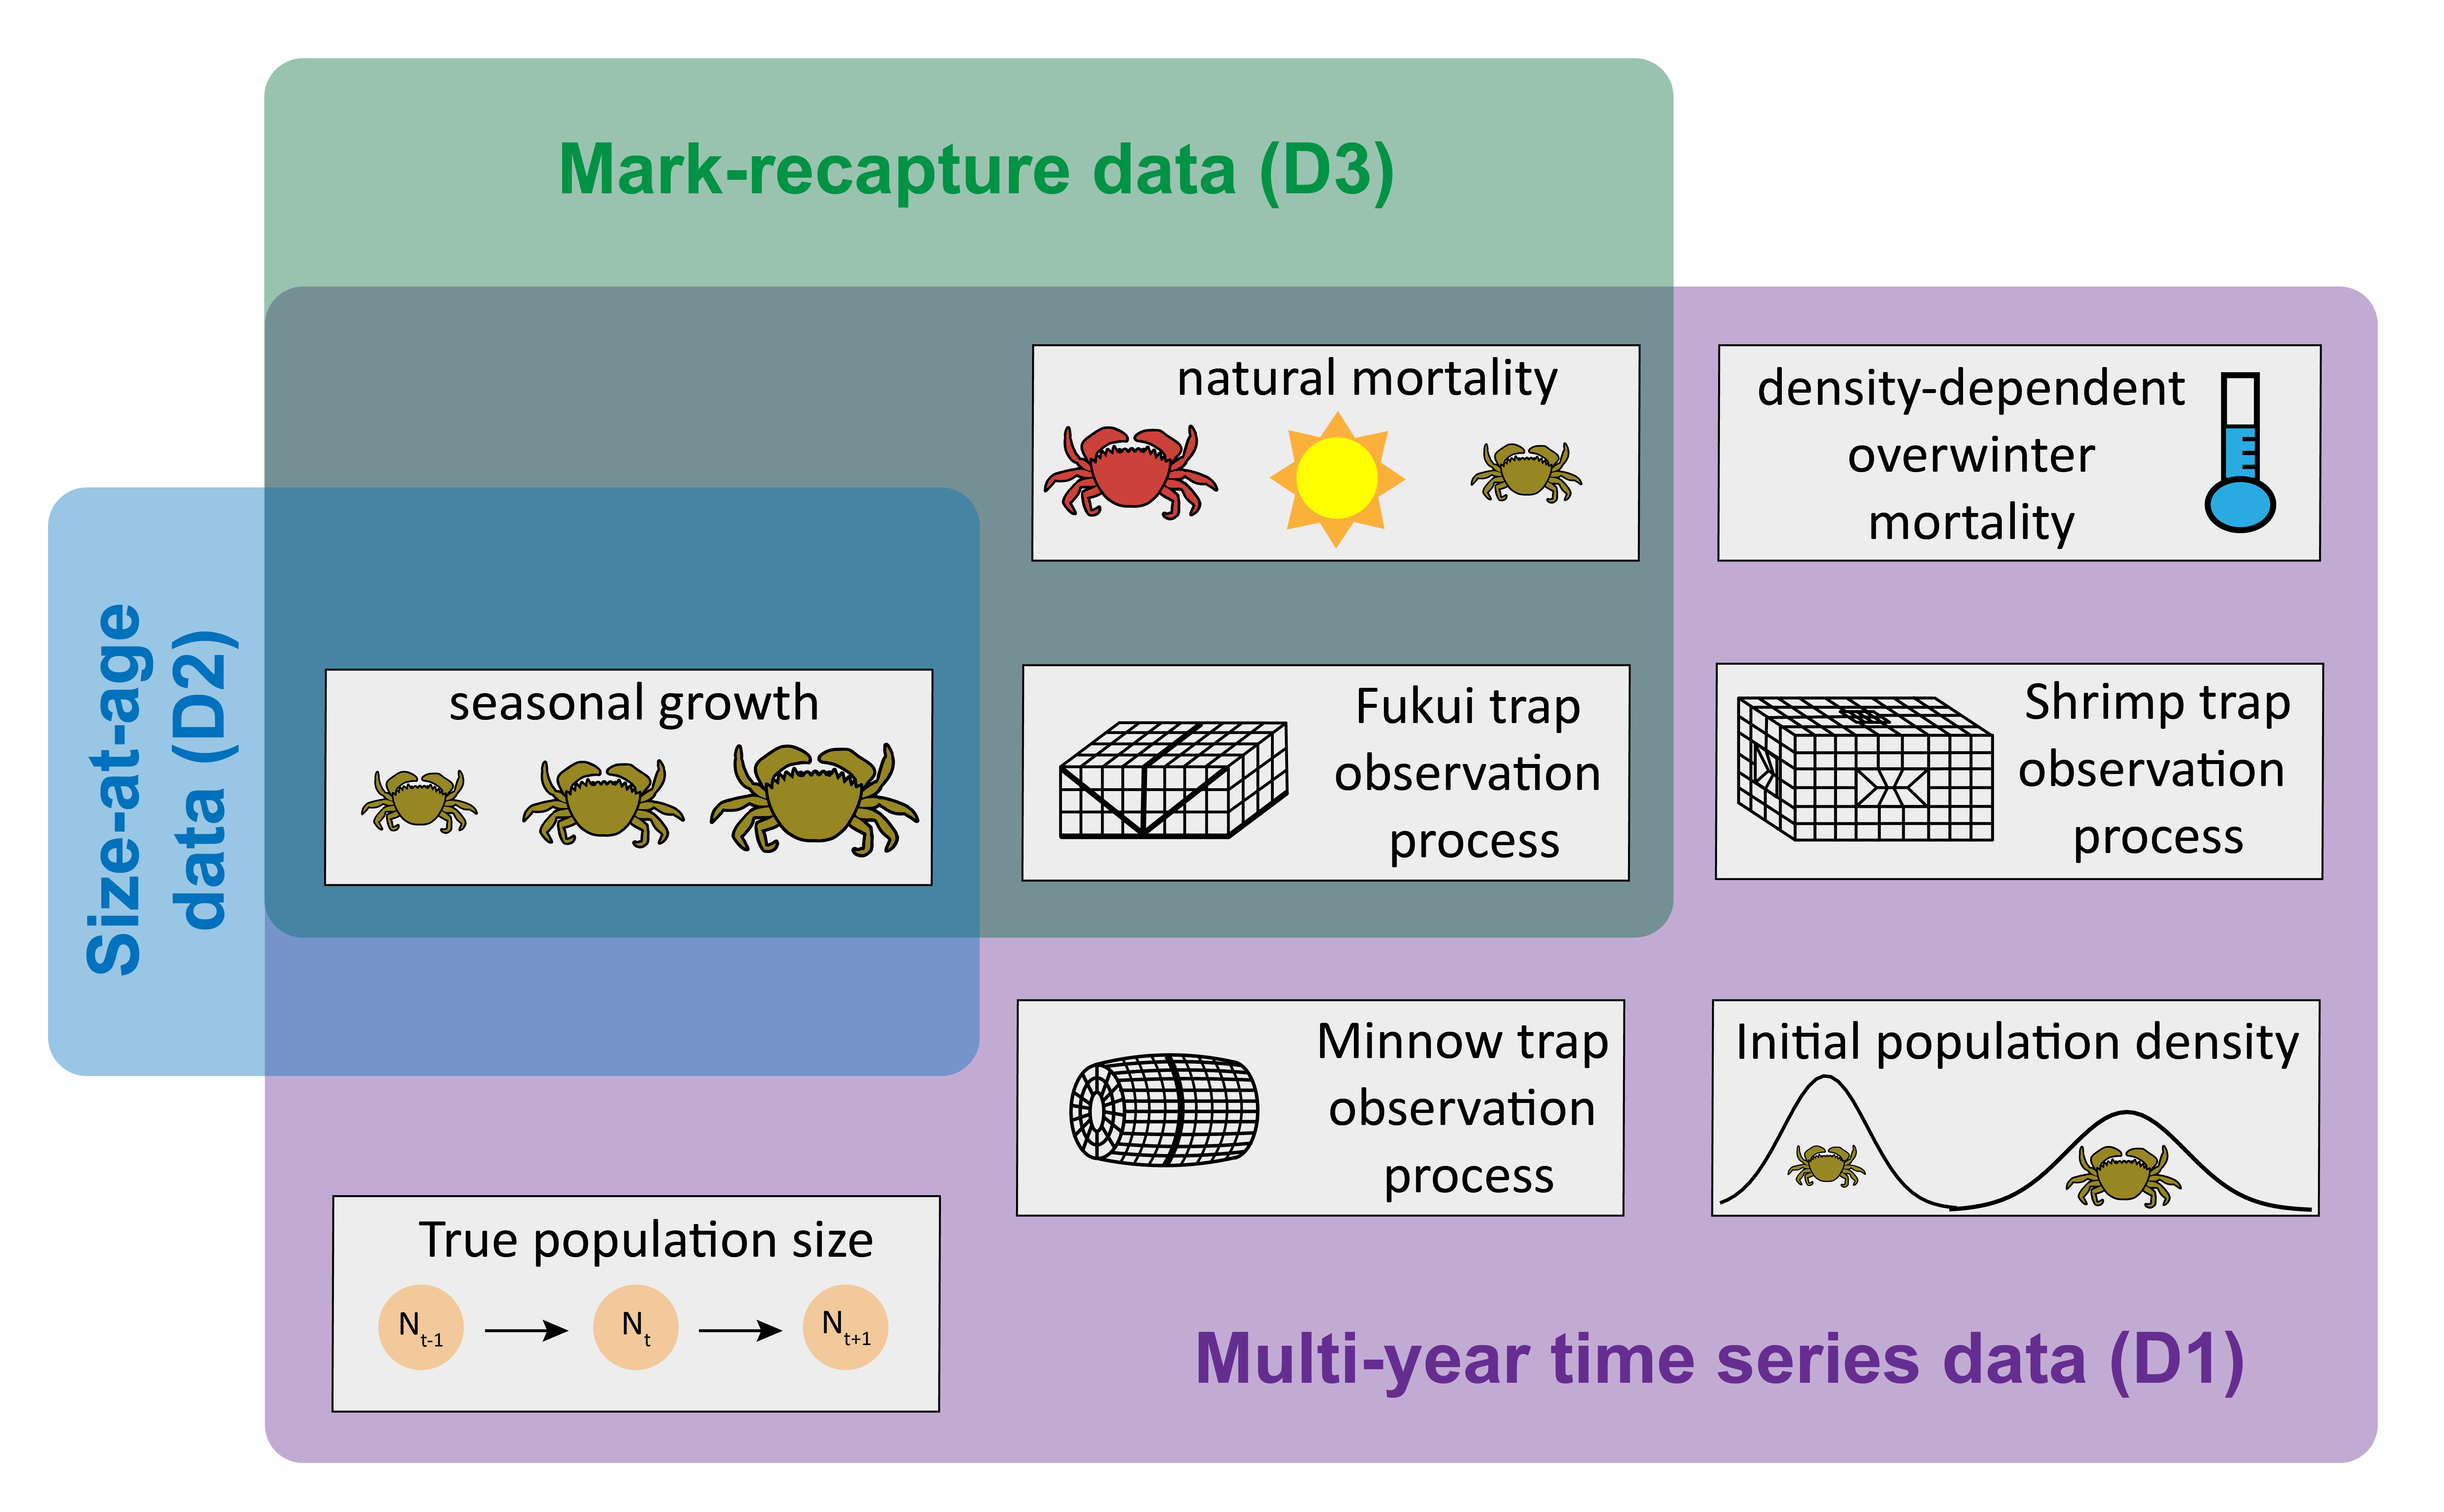
\includegraphics[width=1\textwidth]{Figure2_IPM_conceptual-01.png}
    \caption{Overview of parameters informed by the three datasets in the integrated population model: time series data (D1) (Figure 1B), size-at-age data (D2) (Figure A1.1), and mark-recapture data (D3). Parameter categories correspond to categories designated in Table 1.}
\end{figure}

\begin{figure}[H]
    \centering
    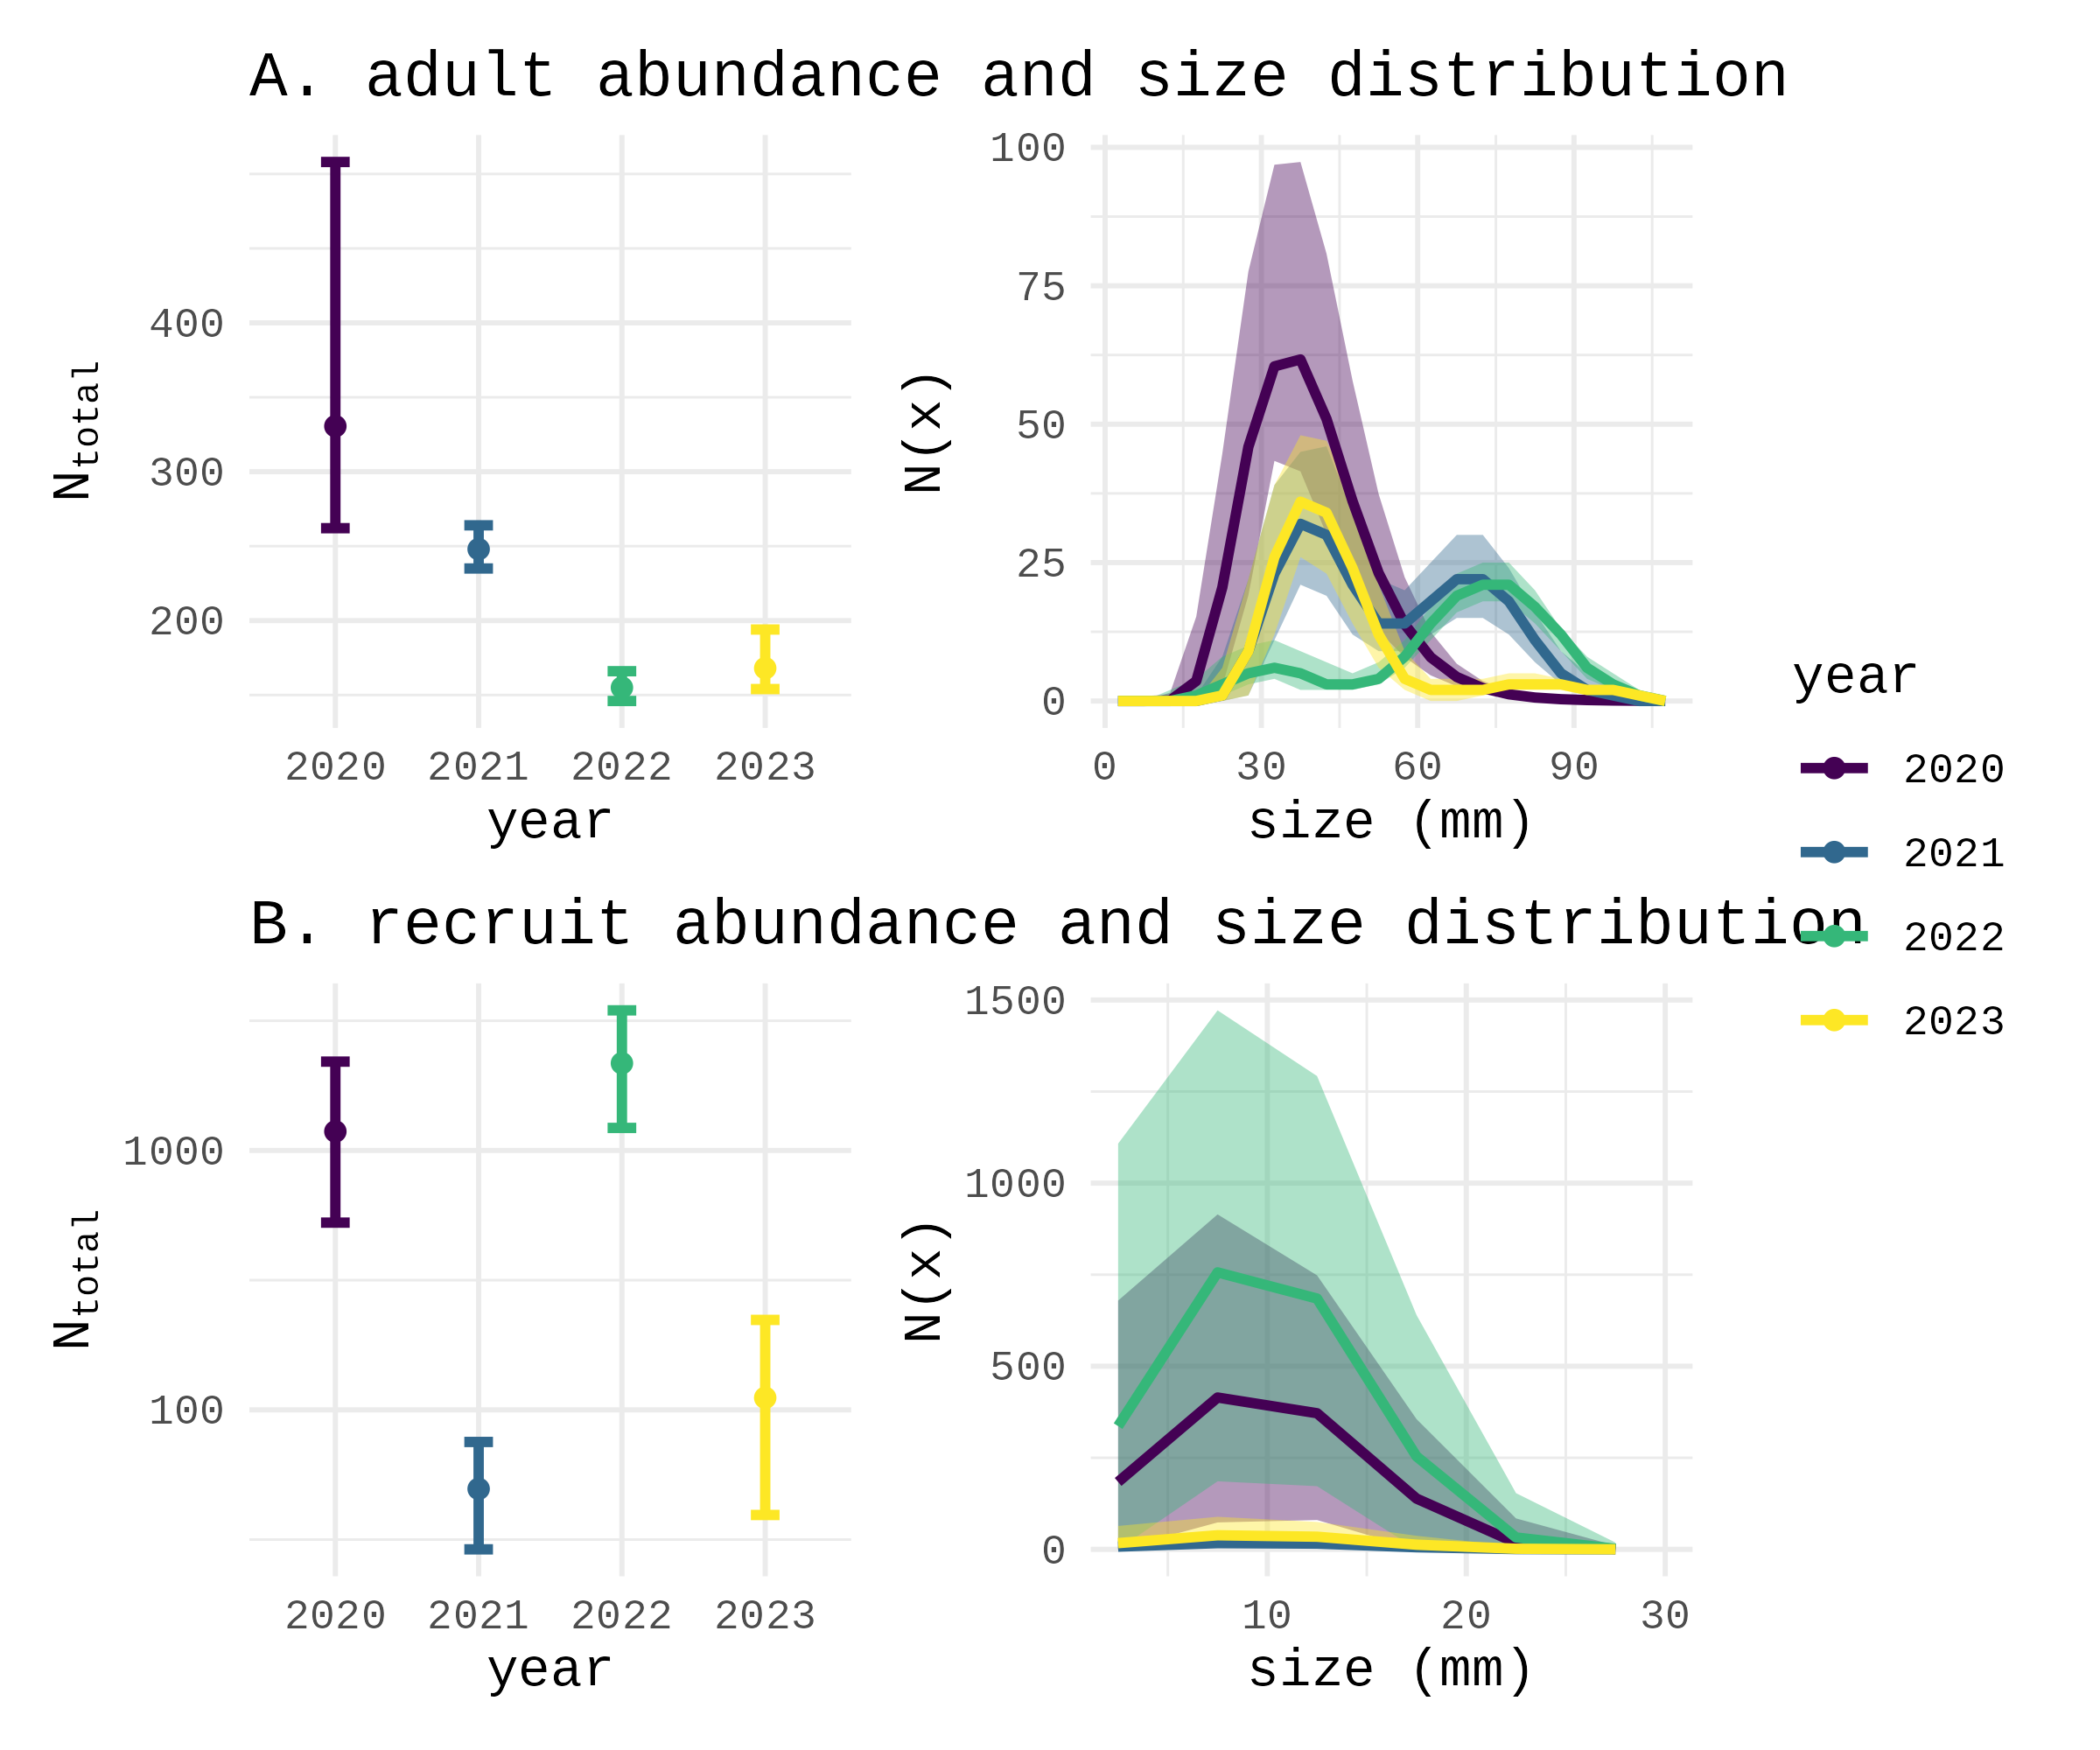
\includegraphics[width=1\textwidth]{Figure3_abundance_sizedist.png}
    \caption{Total abundance and size distribution of \textit{A.} adults and \textit{B.} recruits. The left panels show the size distribution, or the number of individuals in each size class, $N_{size}$. The right panels show the total abundance of crabs across all size classes, $N_{total}$, in each year. Colors indicate the year, and error bars indicate the 95\% credibility interval. Note that the right panel is the integral of the left panel.}
\end{figure}

\begin{figure}[H]
    \centering
    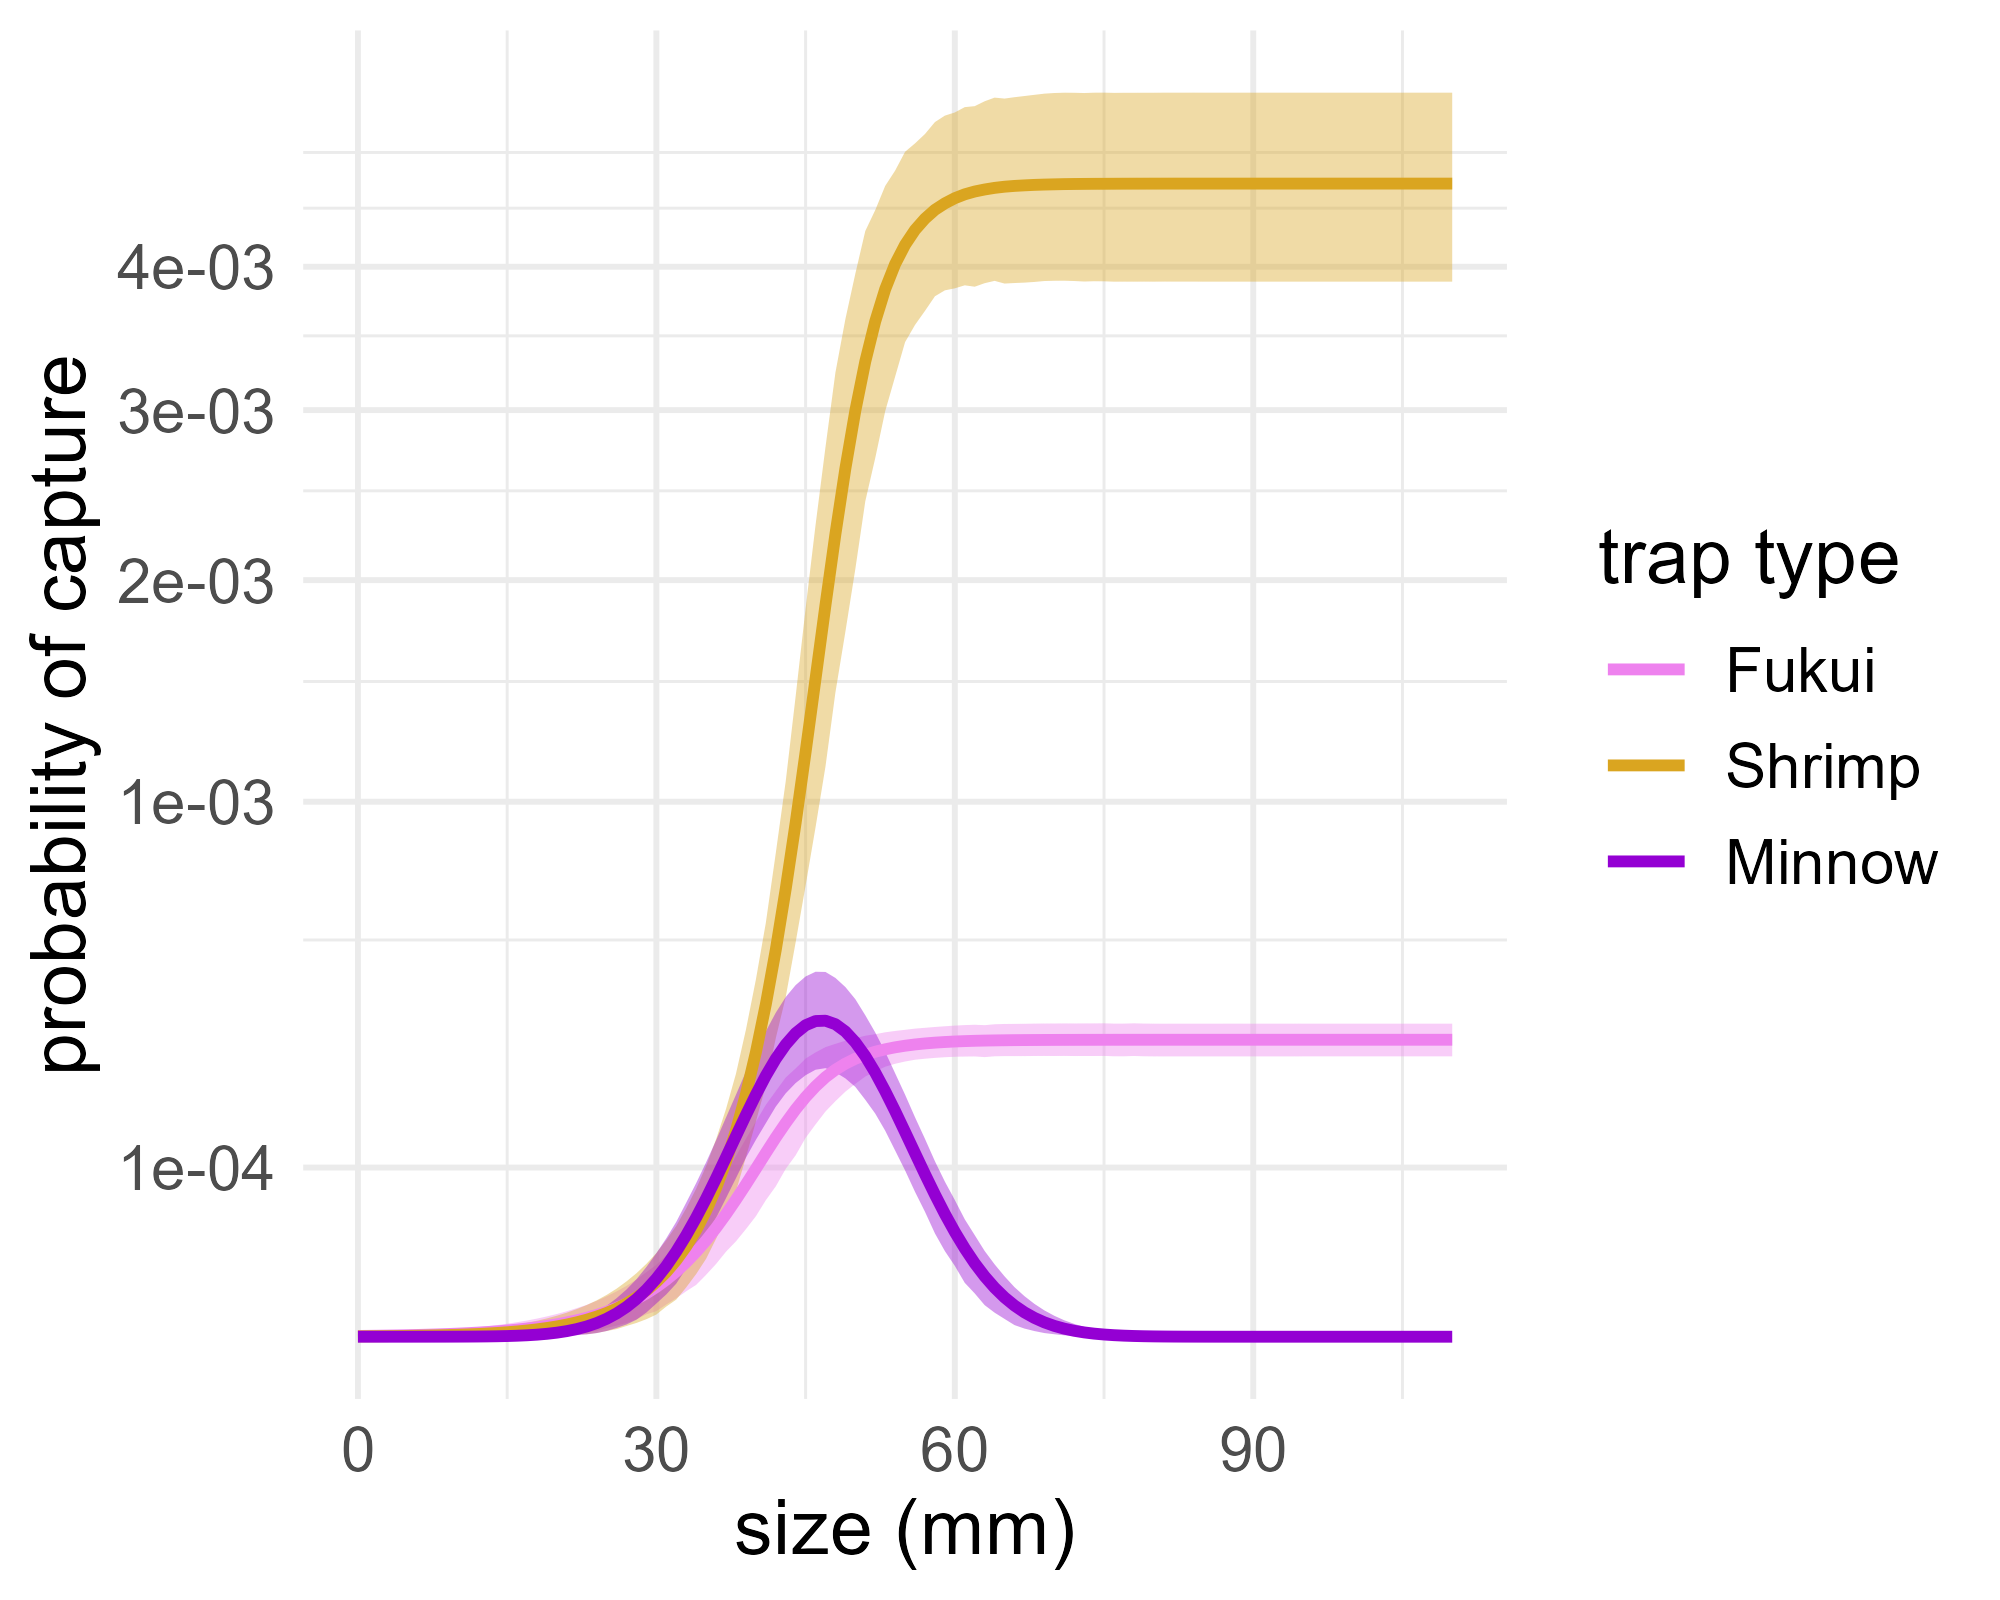
\includegraphics[width=0.8\textwidth]{Figure4_sizesel.png}
    \caption{Size-structured probability of capture, $p_{y}$, in one trap over a 24 hours trapping period. Colors indicate the trap type. Note that the y-axis is presented with a square root transformation.}
\end{figure}

\begin{figure}[H]
    \centering
    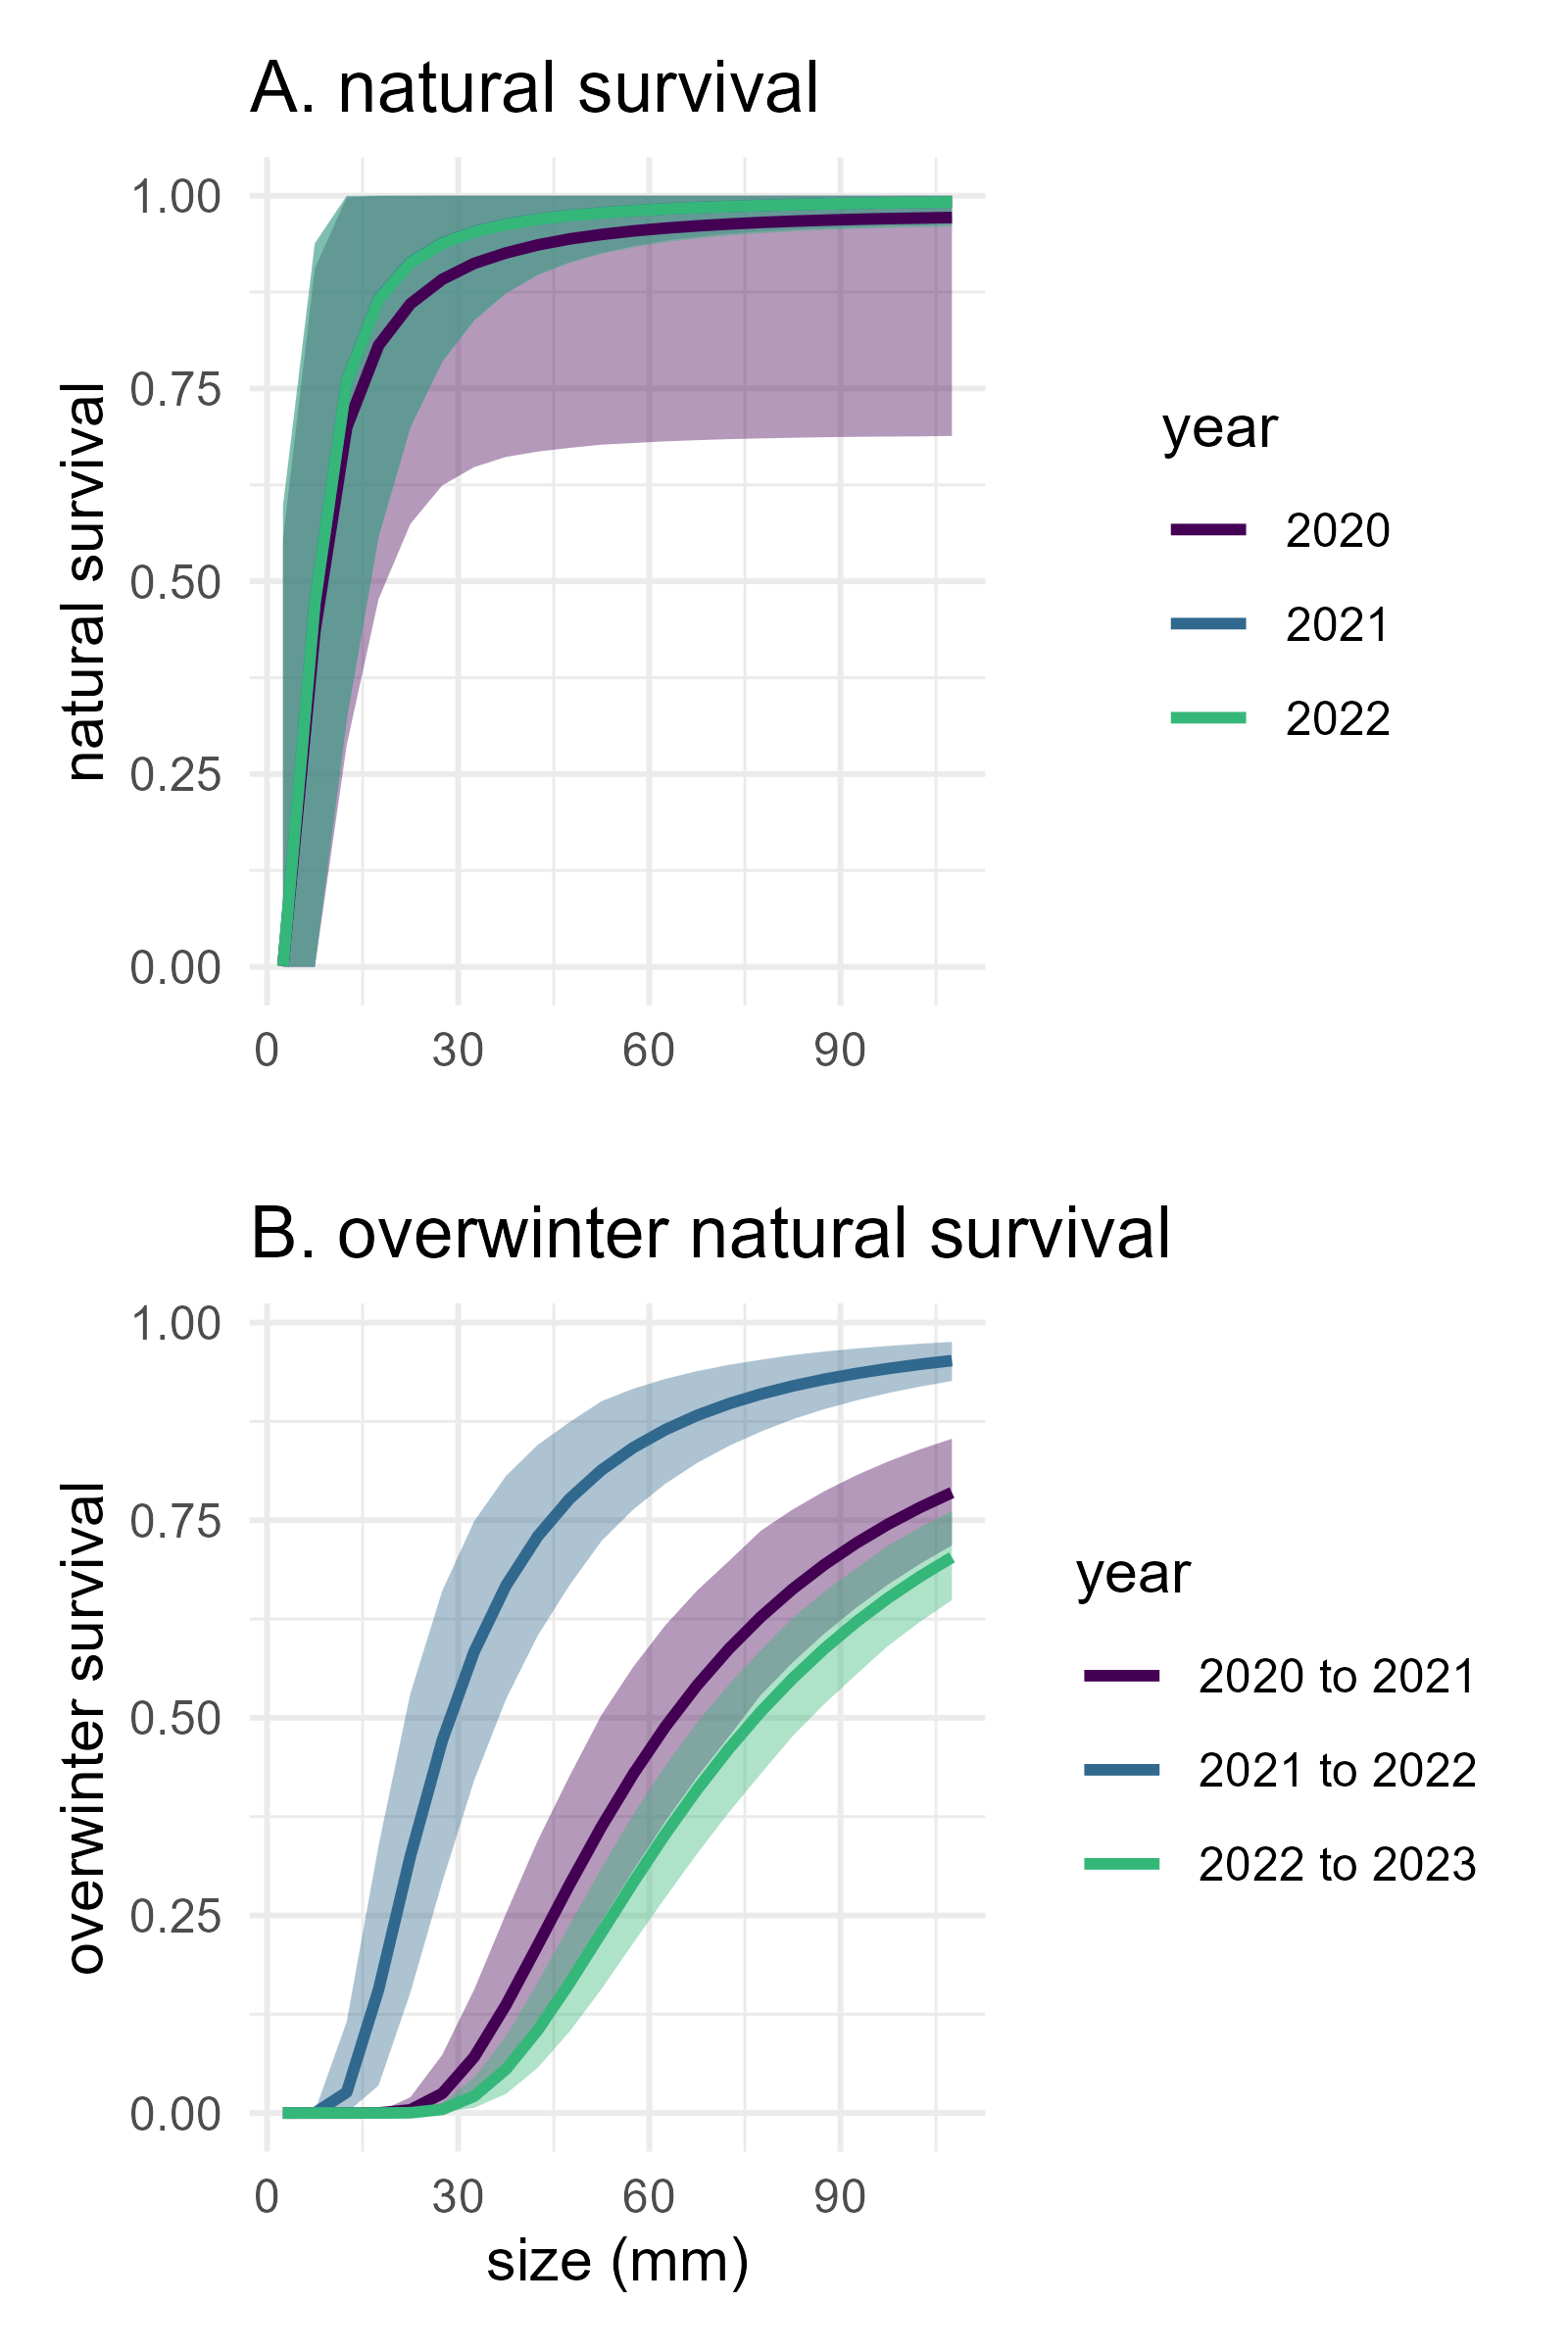
\includegraphics[width=0.7\textwidth]{Figure5_survival.png}
    \caption{Size-structured natural survival rate in the \textit{A.} non-winter season between Julian days 91 and 305 (Eq. 11) and \textit{B.} overwinter (Eq. 15) between Julian day 306 and Julian day 90 of the following year. Colors indicate year, and error bars indicate the 95\% credibility interval.}
\end{figure}

\begin{figure}[H]
    \centering
    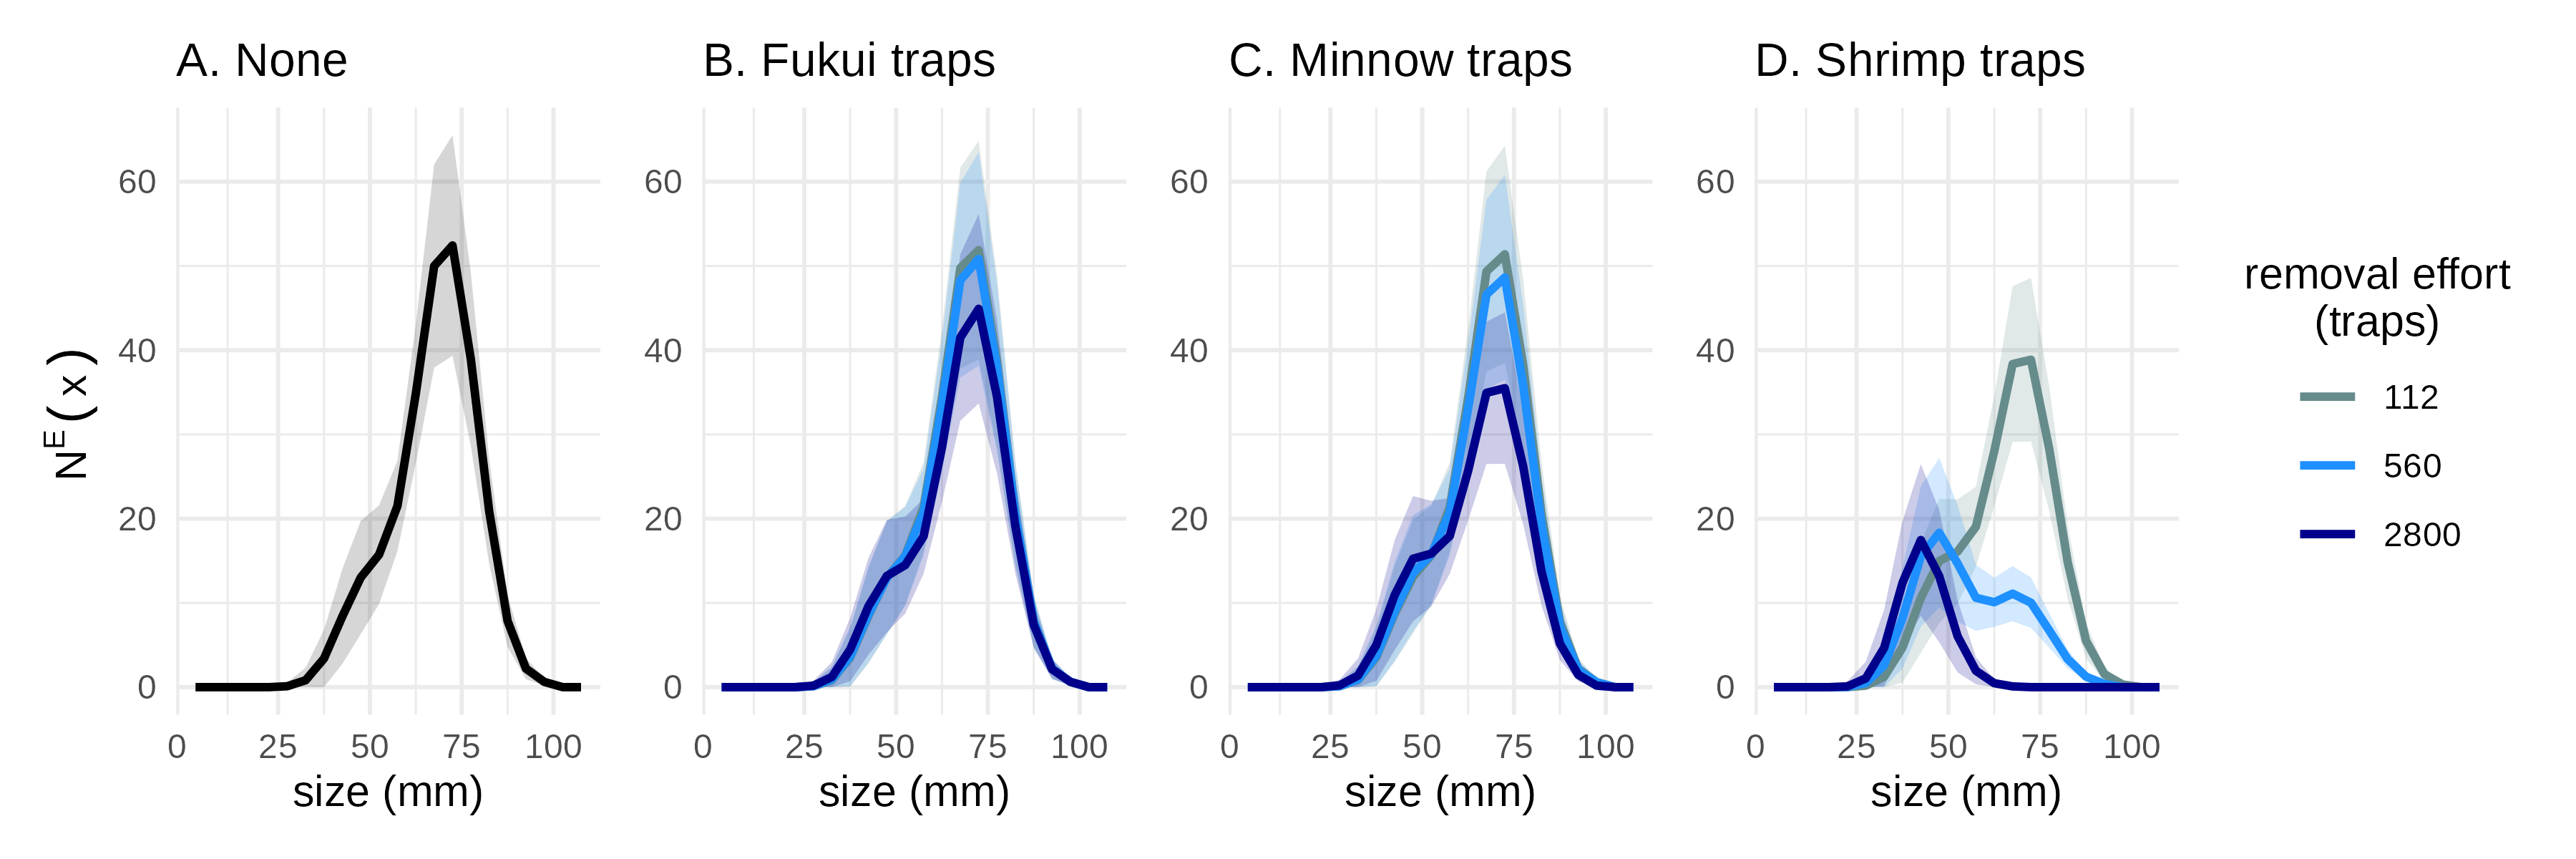
\includegraphics[width=1\textwidth]{Figure6_IPM_simulations.png}
    \caption{Population forecasts in response to varying removal efforts. Size distributions show the crab abundance in each size class, $N_{size}$, at the end of the year after overwinter mortality when \textit{A.} 0 traps, \textit{B.} 112 traps, \textit{C.} 560 traps, and \textit{D.} 2800 traps were applied evenly over a trapping season of 14 biweeks. Solid line indicates the median size-structured abundance across simulation replicates, and the shaded area indicates $\pm1$ standard deviation across simulation replicates. Colors indicate trap type used (i.e., in panel B, the purple line shows the resulting size distribution after a trapping effort of 112 Minnow traps).}
\end{figure}

\section{Acknowledgements}

We thank Sylvia Yamada, Ted Grosholz, Brian Turner, and Tom Therriault for providing valuable feedback on European green crab population dynamics and model development; Northwest Straits Commission and Washington Department of Fish and Wildlife for data collection and management.  

\printbibliography[]

\end{document}
